
\section{Research Interests \& Experience}


\begin{frame}{\underline{\secname}}


\begin{center}
\textbf{GANs to simulate Drell-Yan  events in  ATLAS experiment}
\end{center}

\begin{itemize}			  \setlength\itemsep{0em}

\item GAN: A two- Deep NN game where one genrate events (generator) and one (discriminator) classifies events as real (from real simulation ) or fake (from the generator)

\item the game ends when the generator success to fool the discriminator = the generator can produce events similar to a real simulation

\item GANs can learn complex P(x)

\item GANs provide a viable strategy for speeding up numerically intensive simulation

\end{itemize}
\begin{figure}[H]
\begin{center}
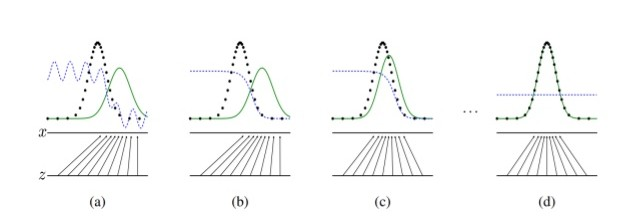
\includegraphics[width=0.6\textwidth]{figures/gauss.jpg}
\end{center}
\end{figure}

\end{frame}



\begin{frame}{\underline{\secname}}


\begin{center}
\textbf{Preparing the dataset}
\end{center}
\begin{itemize}			  \setlength\itemsep{0em}

\item
Considering a sample of $Z \to \mu \mu$ events in proton-proton collisions,
\item
generated using the {\tt PYTHIA8} event generator at a center-of-mass energy of 13~TeV.
\item
Detector resolution and efficiency are taken into account using the parametric description of the ATLAS detector provided by the {\tt DELPHES} detector simulation library.
\item
Events are generated with an average of 20 simultaneous collisions (pileup)
\item \textbf{Problems} : Choosing the number of features - choosing coordinate system - finding the best GAN structure

\end{itemize}

\end{frame}



\begin{frame}{\underline{\secname}}

%A rotation of the two four-momenta is applied, so that $p_y^{\mu 1}=0$, after the rotation. Once this is done, $p_y^{\mu 1}$ is discarded from the dataset.

\begin{center}
\textbf{Preparing the dataset}
\end{center}

\begin{figure}[H]
\begin{center}
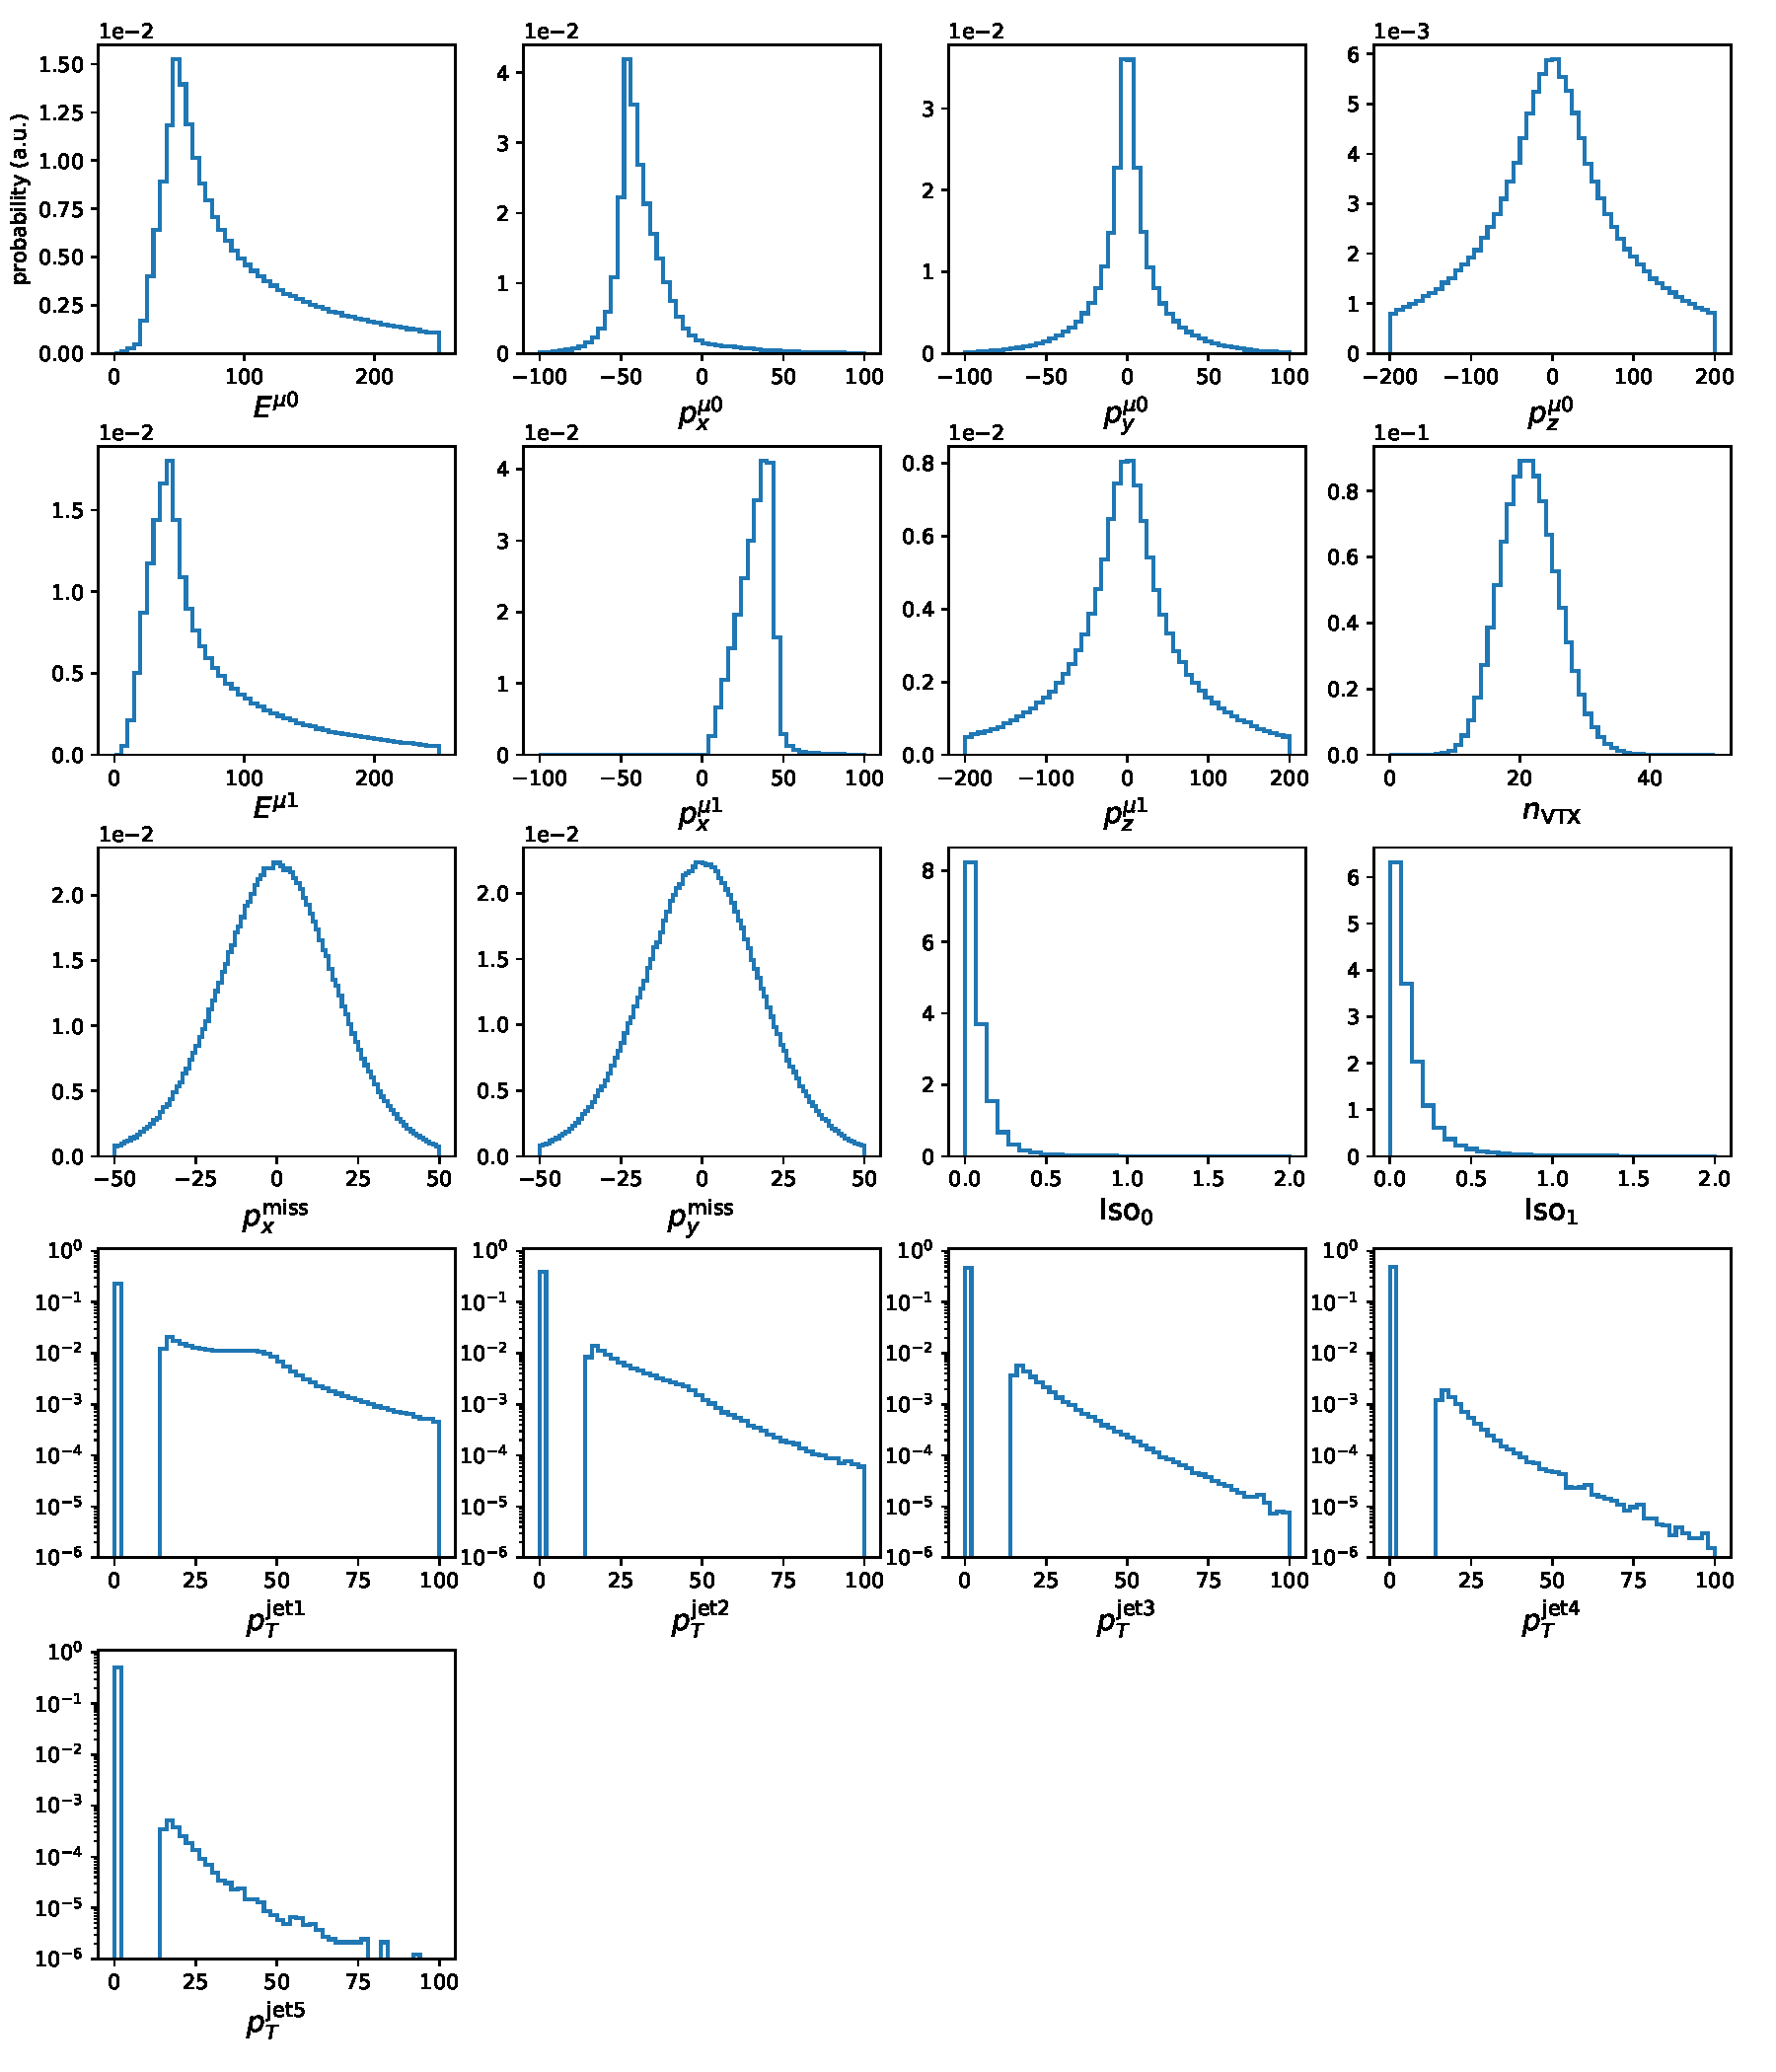
\includegraphics[width=0.4\textwidth]{slides/plotmatrix_realonly_train}
\end{center}
\end{figure}

\end{frame}


\begin{frame}{\underline{\secname}}

%A rotation of the two four-momenta is applied, so that $p_y^{\mu 1}=0$, after the rotation. Once this is done, $p_y^{\mu 1}$ is discarded from the dataset.

\begin{center}
\textbf{Final dataset}
\end{center}

\begin{figure}[H]
\begin{center}
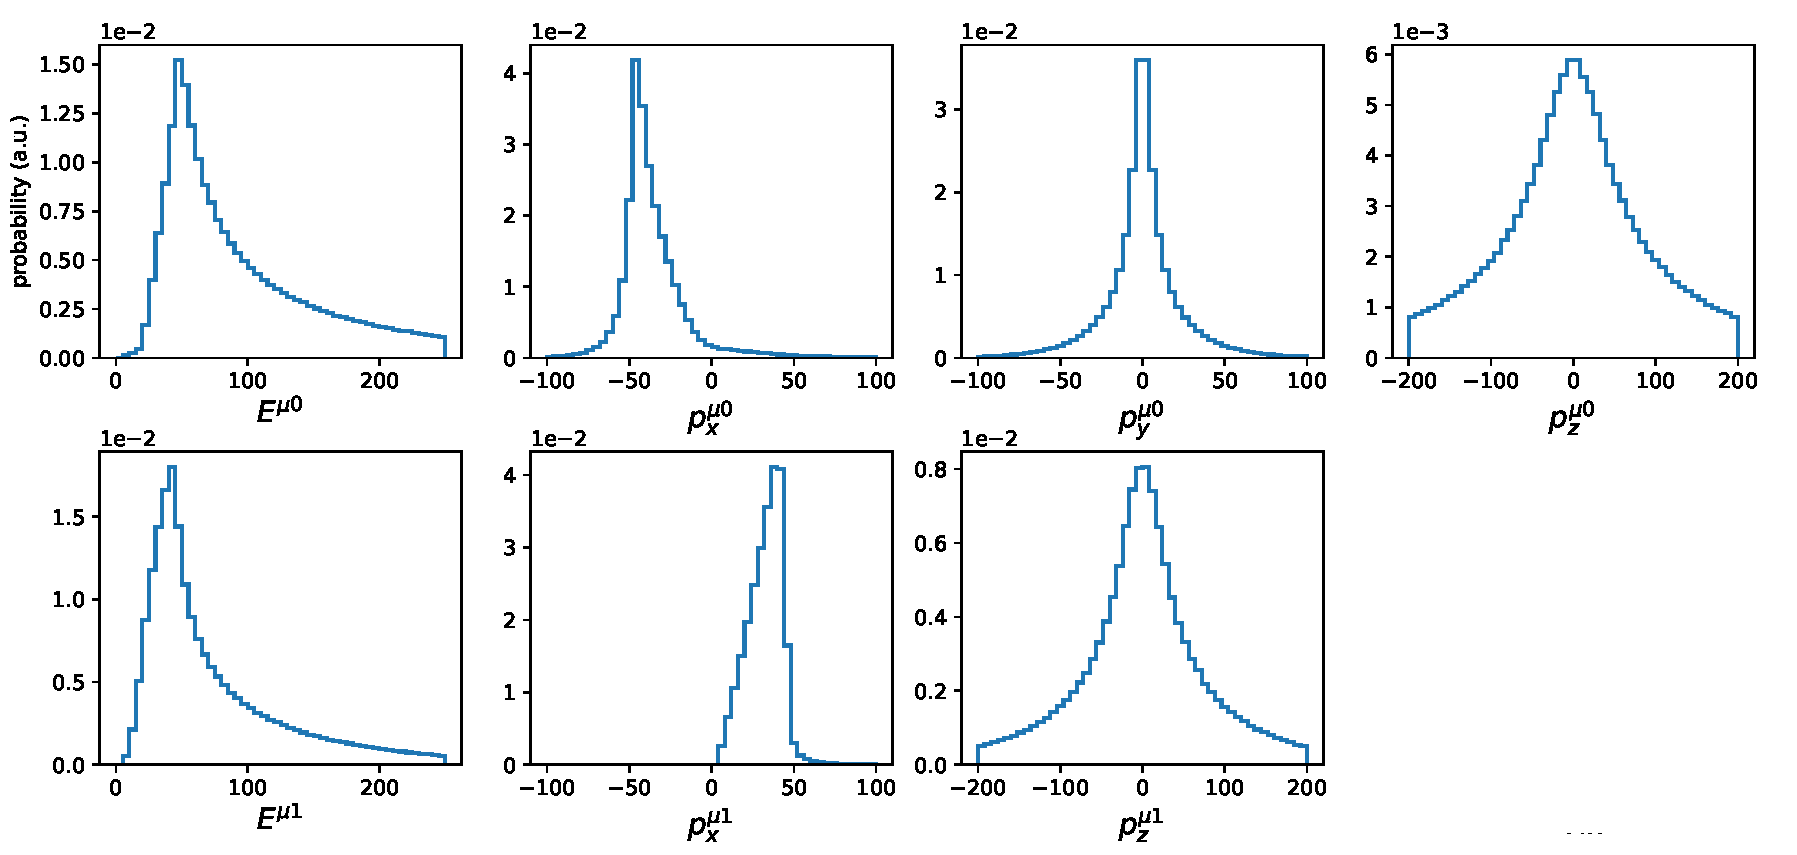
\includegraphics[width=\textwidth]{slides/pdfresizer.com-pdf-crop}
\end{center}
\end{figure}

\end{frame}

\begin{frame}{\underline{\secname}}

\begin{center}
\textbf{The GAN structure}
\end{center}
\begin{itemize}			
\item

The generator network consists of 7 fully connected layers, The input to the generator network consists of 7 ``noise'' floating-point numbers, sampled from a Gaussian distribution centered at 0 with unit variance.
% Neurons in the inner layers are activated by leaky ReLU functions, while linear activation functions are used for the output layers. 


\item

The discriminator network consists of 9 hidden dense layers % with 128, 128, 256, 256, 128, 64, 32, 16, and 8 neurons, activated by a leaky ReLU function. The last hidden layer is fully connected to a single-neuron output layer with sigmoid activation. In addition, a layer connected directly to the input layer returns the dilepton mass as part of the output.

\item

The combined network is trained adversarially for 40,000 epochs.

\item

All networks were implemented in {\tt KERAS}, using {\tt TensorFlow} as a back-end, The training was performed using Google TPU type (v2).

\end{itemize}

\end{frame}


\begin{frame}{\underline{\secname}}


\begin{center}
\textbf{The GAN structure}
\end{center}

\begin{center}
{The generator network}
\end{center}
\begin{figure}[H]
\begin{center}
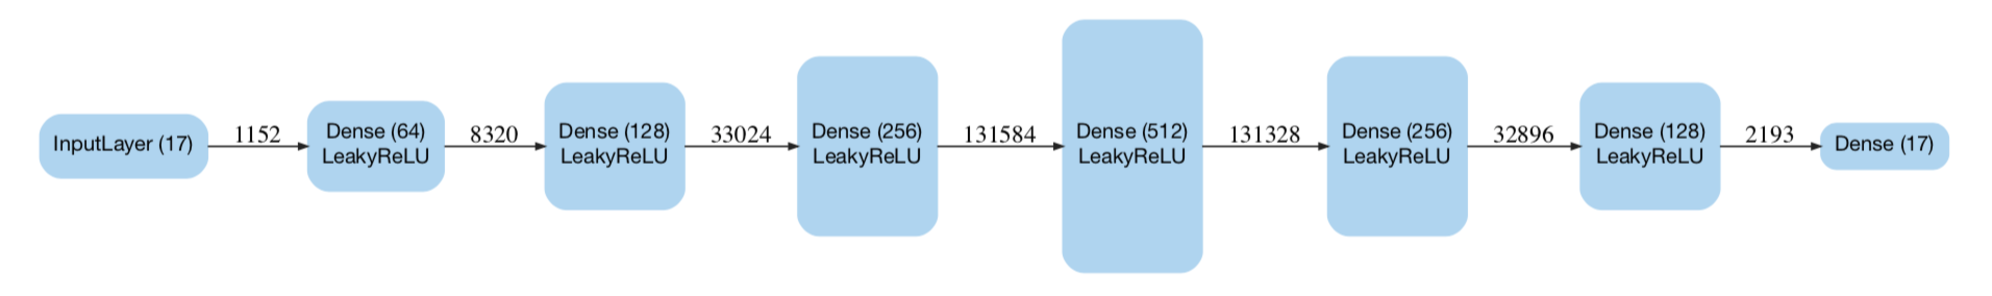
\includegraphics[width=\textwidth]{slides/generator_network}
\end{center}
\end{figure}

\begin{center}
{The discriminator network}
\end{center}

\begin{figure}[H]
\begin{center}
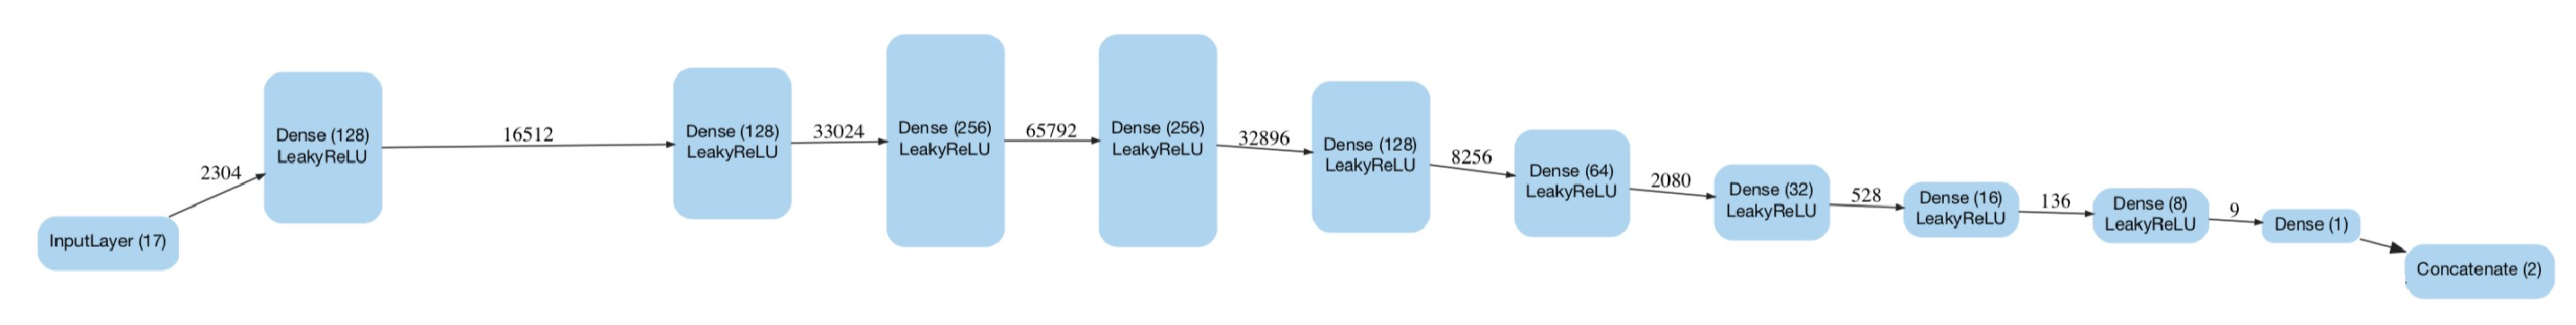
\includegraphics[width=\textwidth]{slides/discriminator_network}
\end{center}
\end{figure}

\end{frame}

\begin{frame}{\underline{\secname}}


\begin{center}
\textbf{Results}
\end{center}


\begin{figure}[H]
\begin{center}
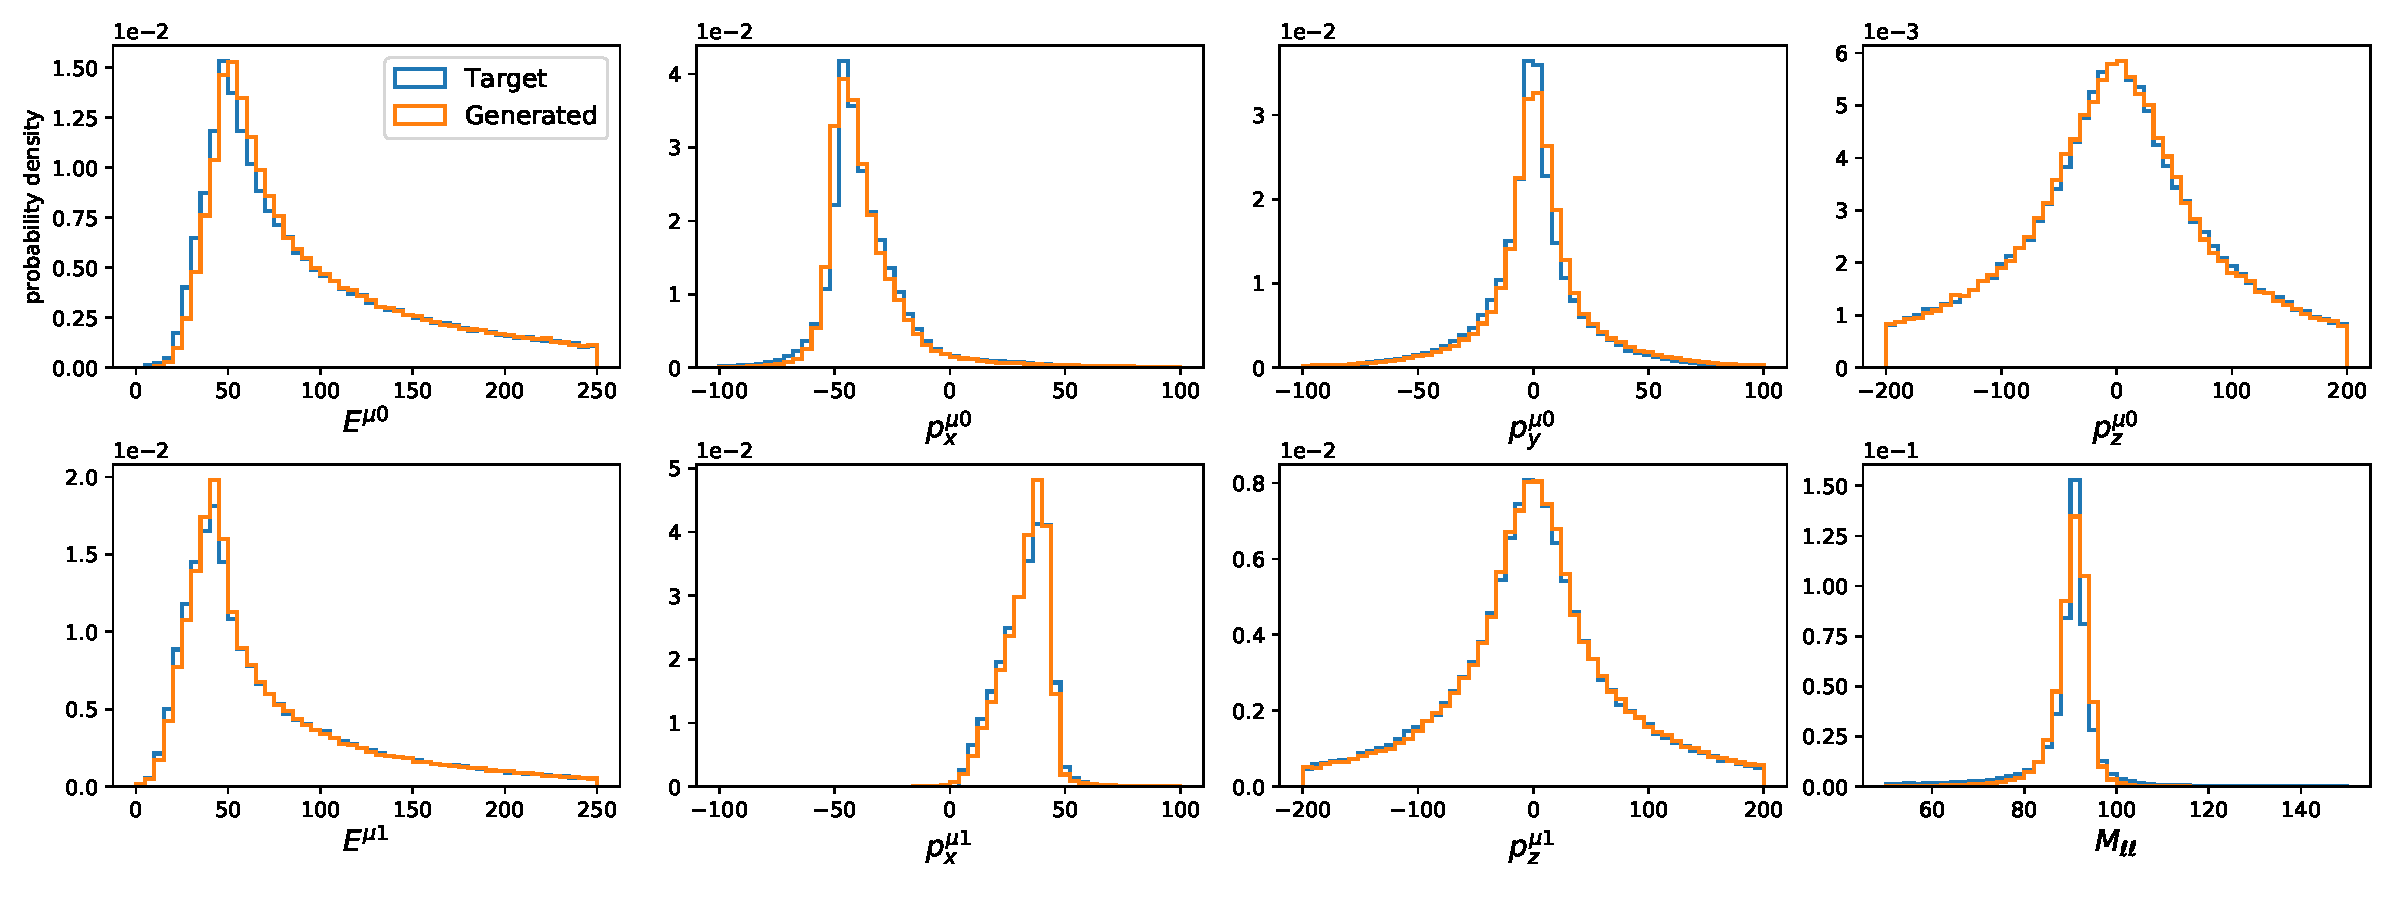
\includegraphics[width=\textwidth]{slides/trial9_epoch39700_minigantest_mllloss_final}
\end{center}
\end{figure}





\end{frame}

\begin{frame}{\underline{\secname}}


\begin{center}
\textbf{Results}
\end{center}

\begin{itemize}			  \setlength\itemsep{0em}
\item \textbf{GAN} : 5000 events/s  \t{  } \textbf{{\Large $ <<  $}}\t{  }  \textbf{DELPHES + Pythia} : 5000 events in \textit{{$\sim 3.5$ min}}
\item
Results show that GANs can learn the multi-dimensional pdf of $\cal{O}$(7) features
\item
The GAN shows problems in learning distributions with sharp features such as edges
\item
The Gan indicate a good performance but the reached precision is still insufficient to meet the precision requirements of an LHC data analysis.
\end{itemize}

\begin{center}
\textbf{Solutions}
\end{center}
\begin{itemize}			  \setlength\itemsep{0em}
\item Auxiliary GAN
\item reinforcement learning

\item  Conditional Hybrid GAN


\end{itemize}
\end{frame}
%
%\begin{frame}{\underline{\secname} : Other computational Projects}
%	\begin{columns}
%		\begin{column}{0.5\linewidth}
%
%	\begin{itemize}			  \setlength\itemsep{0em}
%		\item \textbf{Higgs ML }: signal / background separation using RNN and Xgboost instead of BDT
%		\item \textbf{Epidemic simulation} : a simulation using Pygame to show people why they need to stay at home and help Flattening the curve
%		\item \textbf{Also} : websites using Javascript \& ml modules using Python \& open source projects
%		
% 
%\end{itemize}
%		\end{column}
%
%		\begin{column}{0.5\linewidth}
%
%			
%			% \animategraphics[loop,width=\textwidth]{10}{slides/New Folder/something-}{0}{16}
%
%			\begin{figure}[H]
%				\begin{center}
%					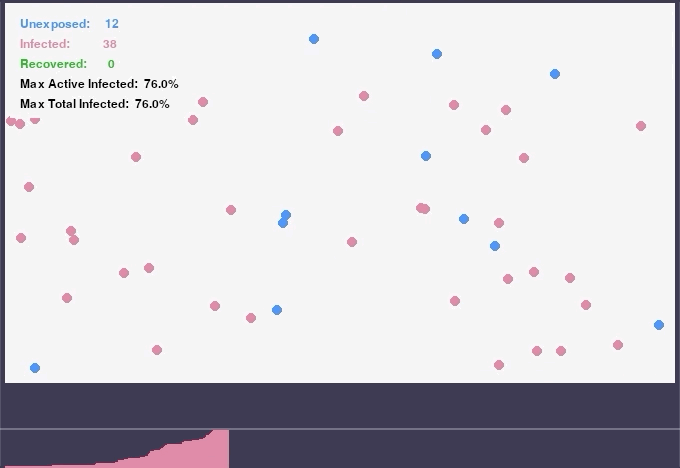
\includegraphics[width=\textwidth]{slides//New Folder/something-70}
%				\end{center}
%			\end{figure}
%		
%
%
%		\end{column}
%	\end{columns}
%
%\end{frame}





